\documentclass[conference]{IEEEtran}
\IEEEoverridecommandlockouts
% The preceding line is only needed to identify funding in the first footnote. If that is unneeded, please comment it out.
\usepackage{cite}
\usepackage{amsmath,amssymb,amsfonts}
\usepackage{algorithmic}
\usepackage{graphicx}
\usepackage{textcomp}
\usepackage{xcolor}
\usepackage{enumitem}
\def\BibTeX{{\rm B\kern-.05em{\sc i\kern-.025em b}\kern-.08em
    T\kern-.1667em\lower.7ex\hbox{E}\kern-.125emX}}
\begin{document}

\title{Asteroseismology: AI-Driven Seismic Event Detection for Extra-Terrestrial Missions\\
}

\author{\IEEEauthorblockN{Muhammad Zain Ali}
    \IEEEauthorblockA{\textit{Dept. of Physics} \\
        \textit{Quaid-i-Azam University}\\
        Islamabad, Pakistan \\
        zain@betelwise.com}
    \and
    \IEEEauthorblockN{Khabab Nazir}
    \IEEEauthorblockA{\textit{Dept. of Physics} \\
        \textit{Quaid-i-Azam University}\\
        Islamabad, Pakistan \\
        khababnazir10@gmail.com}
}

\maketitle

\begin{abstract}
    Planetary seismology faces significant challenges in transmitting continuous seismic data due to bandwidth and power
    constraints. Traditional event detection methods generate numerous false positives, leading to inefficient data
    transmission. This paper presents Asteroseismology, an AI-enhanced seismic event detection framework that integrates
    classical phase-picking algorithms with machine learning to optimize seismic data processing for space missions. The
    workflow begins with automatic bandpass filtering, outlier removal, and normalization to enhance signal clarity. A
    Short-Term Average to Long-Term Average (STA/LTA) analysis is then applied to detect candidate events, followed by a
    filtering mechanism that refines initial picks based on characteristic function slopes. The final step employs a
    Convolutional Neural Network (CNN), trained on seismic data from the Apollo Lunar Surface Experiments Package
    (ALSEP) and NASA’s Mars InSight mission, to distinguish true seismic events from noise, ensuring high precision
    while minimizing false detections. Designed for computational efficiency, the system processes a month’s worth of
    seismic data in under 60 seconds on an average processor. It also features six tunable parameters, allowing
    adaptation to different planetary environments and mission constraints. Initial results demonstrate that the CNN,
    despite limited training, achieves over 80 percent event detection accuracy with a false positive rate of
    approximately 5 percent. Future enhancements include refining the CNN within an Auxiliary Classifier Conditional GAN
    (AC-GAN) framework to further improve detection reliability. This AI-driven approach enables autonomous seismic data
    analysis onboard spacecraft, significantly reducing the need for raw data transmission and paving the way for more
    efficient planetary and lunar seismology missions.
\end{abstract}

\begin{IEEEkeywords}
    Seismic Event Detection, Planetary Seismology, Machine Learning,
    CNN, STA/LTA, AI in Space Exploration.
\end{IEEEkeywords}

\section{Introduction}
    The seismic exploration of planetary bodies like the Moon and Mars is fundamental to understanding their internal
    structure, geological evolution, and potential for past or present habitability \cite{Lognonne2005, Lognonne2019}.
    Data from missions such as the Apollo Passive Seismic Experiment (PSE) \cite{Nakamura1982} and the ongoing Mars
    InSight mission with its SEIS instrument\cite{Lognonne2019} have provided invaluable windows into these worlds. A
    primary constraint in planetary seismology, as emphasized by \cite{Civilini2021}, is the costly power and bandwidth
    requirements associated with delivering continuous seismic data back to Earth from distant missions.

    A fundamental challenge in planetary seismology is the efficient management and transmission of the vast quantities
    of continuous seismic data generated by lander-based instruments. Deep-space missions operate under severe
    constraints on power, bandwidth, and data volume (Lorenz, 2015, as cited in Civilini et al., 2021; Lognonné et al.,
    2019). For instance, the SEIS instrument on the Mars InSight mission, while typically downlinking continuous data at
    2 samples per second (sps), generates a significant data volume; \cite{Lognonne2019} note that its full data
    generation capability is orders of magnitude larger than its telemetry allocation. \cite{Civilini2021} quantified
    that the telemetry for SEIS consumes approximately 1.5\% of the InSight lander's total power output. If we were to
    consider data rates comparable to those from some Apollo experiments, which utilized sampling rates such as 6.625 Hz
    for the Passive Seismic Experiment (PSE) mid-period instruments \cite{Nunn2020}, the data volume and consequently
    the power required for transmission by a modern system like SEIS would consume an even more substantial portion of a
    lander's available power. Extrapolating further, \cite{Civilini2021} projected that a similar seismic setup for a
    mission to Europa could demand 8.8–13.2\% of the lander's power solely for seismic data transmission. These figures
    underscore the critical necessity for sophisticated on-board data processing and event detection algorithms to
    prioritize scientifically valuable data segments for downlink, thereby making the most efficient use of limited
    mission resources.

    Traditional automatic event detection algorithms, like the Short-Term Average to Long-Term Average (STA/LTA) ratio
    (Allen, 1982, as cited in \cite{Civilini2021}), while computationally inexpensive, often struggle with the low
    signal-to-noise ratios and complex noise environments encountered on planetary surfaces. This can lead to a high
    rate of false positives, thereby inefficiently utilizing the scarce telemetry resources \cite{Civilini2021}.
    Furthermore, the unique characteristics of seismic wave propagation on bodies like the Moon, with its highly
    scattering near-surface layer leading to prolonged codas \cite{Dainty1981, Nakamura1982} , make robust event
    detection and phase-picking particularly challenging.

    In response to these challenges, machine learning (ML) approaches, especially deep learning techniques like
    Convolutional Neural Networks (CNNs), have gained traction in planetary science. \cite{Civilini2021} effectively
    demonstrated that CNNs, trained on spectrograms of Earth-based seismic events and utilizing transfer learning, could
    accurately catalog moonquakes from Apollo PSE and LSPE data, even in the absence of extensive local training
    datasets. This work underscored the potential of ML to generalize from available data and perform robust
    classification.

    This paper introduces "Asteroseismology," an AI-enhanced seismic event detection framework specifically designed to
    address the data optimization needs of extra-terrestrial missions. Our framework uniquely integrates a pipeline of
    classical phase-picking algorithms with a lightweight CNN. This hybrid approach begins with conventional signal
    conditioning, including automatic bandpass filtering, outlier removal, and normalization. Candidate seismic events
    are then identified using STA/LTA analysis, followed by a novel filtering stage based on characteristic function
    slopes to refine these initial picks. The core innovation lies in then feeding these refined candidate events,
    represented as 1D waveform segments augmented with auxiliary statistical features, into a CNN. This CNN, trained on
    a diverse dataset including lunar data from the Apollo missions and Martian data from the InSight mission, is tasked
    with the final discrimination between true seismic events and noise. By leveraging the efficiency of classical
    algorithms for initial data reduction and candidate selection, our system aims to reduce the computational burden on
    the CNN, allowing it to perform high-precision classification. Asteroseismology is designed for computational
    efficiency and adaptability through tunable parameters, making it a strong candidate for future onboard autonomous
    data processing, thereby significantly enhancing the scientific return of planetary seismology missions by
    optimizing precious data transmission resources.

\section{Background}
    The detection of seismic events from continuous waveform data is a fundamental task in seismology. For decades, this
    has been addressed using a variety of algorithmic approaches, evolving from simple amplitude thresholding to more
    sophisticated statistical and pattern recognition techniques.
    \subsection{Lunar Seismology}
        The foundation of extra-terrestrial seismology was laid by the NASA Apollo missions (1969-1977). The Apollo
        Lunar Surface Experiments Package (ALSEP) successfully deployed a network of four primary seismic stations
        (Apollo 12, 14, 15, and 16), complemented by the short-lived Apollo 11 seismometer and the Lunar Seismic
        Profiling Experiment (LSPE) geophone array on Apollo 17 \cite{Nakamura1982, Lognonne2005, Nunn2020}
        %(Nakamura et al., 1981; Lognonné, 2005; Nunn et al., 2020a).
        These Passive Seismic Experiments (PSE) typically included three-component long-period (LP, later referred to as
        mid-period or MP) seismometers and a single-component short-period (SP) seismometer
        \cite{Nunn2020}%(Nunn et al., 2020a).

        Lunar seismic data revealed a surprisingly active Moon, characterized by several types of moonquakes: deep
        moonquakes (DMQs) occurring at depths of 700-1200 km and exhibiting strong tidal periodicities; shallow
        moonquakes (or HFTs - High-Frequency Teleseismic events) at shallower depths (50-220 km); thermal moonquakes
        caused by surface temperature variations; and meteoroid impacts \cite{Nakamura1982, Lognonne2005}
        %(Nakamura et al., 1982; Lognonné, 2005)
        . A key characteristic of lunar seismograms is the intense scattering within the lunar megaregolith, resulting
        in prolonged codas and making phase identification, particularly for S-waves, exceptionally difficult
        \cite{Dainty1981, Garcia2019}
        %(Dainty and Toksöz, 1981; Garcia et al., 2019).

        The initial cataloging of these events, notably by \cite{Nakamura1982}, relied heavily on visual inspection and
        waveform cross-correlation to identify repeating DMQs from distinct source regions or "nests." These efforts
        provided the first constraints on the Moon's internal structure, including its crust, mantle, and the likely
        presence of a small, partially molten core \cite{Weber2011,Garcia2019}
        %(Weber et al., 2011; Garcia et al., 2019).

        More recently, with the digitization and improved accessibility of Apollo data, new analytical techniques have
        been applied. Traditional methods continue to be refined, for example, for re-evaluating Apollo 17 LSPE data
        (Heffels et al., 2017). Machine learning has also begun to make inroads. Knapmeyer-Endrun \& Hammer (2015)
        utilized Hidden Markov Models for event detection in Apollo 16 data. Significantly, Civilini et al. (2021)
        demonstrated the successful application of Convolutional Neural Networks (CNNs), trained on spectrograms of
        Earth-based seismic events via transfer learning, to detect and catalog moonquakes from both PSE and LSPE data.
        This approach highlighted the potential of ML to identify events even with limited or non-local training data,
        by learning characteristic spectral features. Majstorović et al. (2024, preprint/submitted) further explored ML
        by using random forests to classify DMQ source regions based on lunar orbital parameters related to their
        occurrence times, showcasing an approach independent of waveform data for initial source region estimation.

    \subsection{ Martian Seismology}
        Mars has been the focus of renewed seismic interest. The first attempt to place a seismometer on Mars was with
        the Viking landers in 1976. The Viking 2 lander's seismometer, mounted on the lander deck, provided data
        primarily on wind-induced lander vibrations, and only one candidate seismic event was tentatively identified
        \cite{Anderson1977,Lognonne2005}. The on-deck deployment and instrument sensitivity were major limitations.

        Decades later, the NASA InSight mission, which landed in 2018, successfully deployed the SEIS (Seismic
        Experiment for Interior Structure) instrument directly onto the Martian surface \cite{Lognonne2019, Banerdt2020}. 
        %(Lognonné et al., 2019; Banerdt et al., 2020) 
        SEIS comprises a suite of highly sensitive three-component Very Broad Band (VBB) and three-component Short
        Period (SP) seismometers. InSight has definitively recorded hundreds of marsquakes, confirming Mars as a
        seismically active planet \cite{Giardini2020,Clinton2021}. Martian seismic signals, like lunar ones, can be
        influenced by near-surface scattering, though generally less intense than on the Moon. The Marsquake Service
        (MQS) is responsible for ongoing event detection and cataloging, employing a combination of traditional and
        evolving ML-assisted techniques \cite{Clinton2021}.

        %TODO add a section on only CNNs ================================================================

    \subsection{ Machine Learning Paradigms in Seismology }
        The increasing volume and complexity of seismic data from both terrestrial and planetary missions have spurred the
        adoption of machine learning techniques across various seismological tasks. Deep learning, in particular CNNs and
        Recurrent Neural Networks (RNNs), has shown remarkable success in earthquake detection, phase picking, seismic
        imaging, and source characterization on Earth \cite{MousaviBeroza2022}.
        %(Mousavi and Beroza, 2022; Mousavi et al., 2020 - "Earthquake Transformer").

        CNNs are adept at automatically learning hierarchical features from data, making them suitable for analyzing raw
        seismic waveforms or their time-frequency representations (e.g., spectrograms) (Perol et al., 2018; Ross et al.,
        2018b). Generative Adversarial Networks (GANs) have also been explored, for instance, by Li et al. (2018) who
        used a GAN critic as an automatic feature extractor combined with a Random Forest classifier for discriminating
        earthquake P-waves from noise in early warning systems. This highlights the potential of ML to not only classify
        but also to learn compact and effective representations of seismic waves.


\section{Framework}
This framework consists of two core components: an Initial Processing and Candidate
Selection (IPCS) stage leveraging conventional seismic algorithms, followed by a Machine Learning-based Event
Verification (MLEV) stage employing a Convolutional Neural Network (CNN).

The IPCS stage is responsible for initial signal conditioning and candidate event detection from raw seismograms. This
involves a sequence of operations including adaptive bandpass filtering to enhance relevant frequency content, outlier
removal to mitigate transient noise, data normalization for consistent scaling, and STA/LTA analysis to identify
potential seismic onsets. A key feature of this stage is a subsequent refinement step using characteristic function
slope analysis, designed to reduce false positives from the STA/LTA triggers by distinguishing between seismic event
profiles and noise bursts.

Candidate events identified and refined by the IPCS stage are then passed to the MLEV stage. For this stage, rather than
converting waveforms into 2D time-frequency representations, our framework utilizes 1D seismogram segments. These
segments are critically augmented with some auxiliary statistical features, such as standard deviations computed around
the potential arrival times, to provide the CNN with extra contextual information. A lightweight CNN then performs the
final classification, discerning true seismic events from the residual noise and false triggers that have passed the
conventional filtering. This hybrid architecture aims to optimize both computational efficiency and detection accuracy
for planetary missions.
    
    \subsection{Initial Processing and Candidate Events Selection(IPCS)}
    \label{sec:ipcs}
        The Initial Processing and Candidate Selection (IPCS) stage of the framework employs a series of conventional
        seismic signal processing techniques to enhance signal clarity, identify potential seismic events, and reduce
        the number of candidates passed to the subsequent machine learning stage. This stage operates on individual
        seismogram segments loaded from MiniSEED files.
    
        \subsubsection{Adaptive Bandpass Filtering}
            To isolate frequencies most likely to contain seismic signals and attenuate background noise, an adaptive
            bandpass filtering approach is implemented. The system iteratively evaluates a series of predefined
            frequency ranges. For each range, defined by a starting frequency  and a fixed window size , a bandpass
            filter is applied to a copy of the original trace.

            \begin{figure}[htbp]
                \centerline{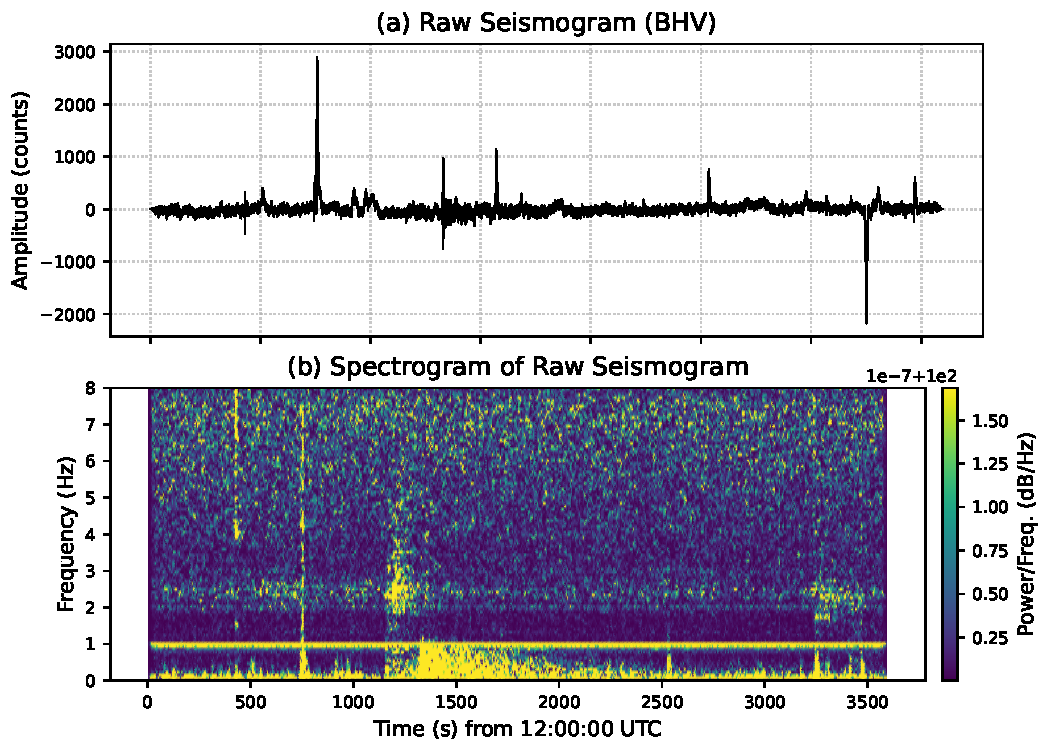
\includegraphics[width=0.9\columnwidth]{figures/fig1_raw_and_spectrogram.pdf}}
                \caption{Example of a raw seismic waveform (top panel) and its corresponding time-frequency 
                spectrogram (bottom panel). This visualization aids in understanding the initial signal 
                characteristics before adaptive filtering.}
                \label{fig:raw_spectrogram_example}
            \end{figure}
            
            The optimal frequency band is determined by one of two methods:
            
            \begin{enumerate}[label=\alph*), leftmargin=3em]
                \item \textit{Power Spectrum Analysis:} The spectrogram of the filtered signal is computed.
                The power values across all frequencies and time points within the spectrogram are flattened, and the average of
                a predefined number (e.g., top 50 or 1000) of the highest power values is calculated. The frequency range
                yielding the maximum average power among these top values is selected as the optimal band. This method
                prioritizes frequency bands where signal energy is most concentrated.
                \item \textit{Standard Deviation Analysis:} The filtered trace data is normalized, and its
                standard deviation is calculated. The frequency range that results in the minimum standard deviation of the
                normalized filtered signal is chosen as the optimal band. This method aims to find a frequency band where the
                signal is most distinct from broadband noise, assuming that a lower standard deviation in a filtered signal
                (after normalization) might indicate a clearer, less noisy signal.
            \end{enumerate}

            The effect of applying the selected adaptive bandpass filter is shown in ``Fig.~\ref{fig:adaptive_filtering_comparison}''
            , which compares the raw seismogram with the seismogram after the optimal bandpass filter has been applied, 
            enhancing the clarity of potential signals within the chosen frequency band.
            % TODO: tell that which example event it is
            \begin{figure}[htbp]
                \centerline{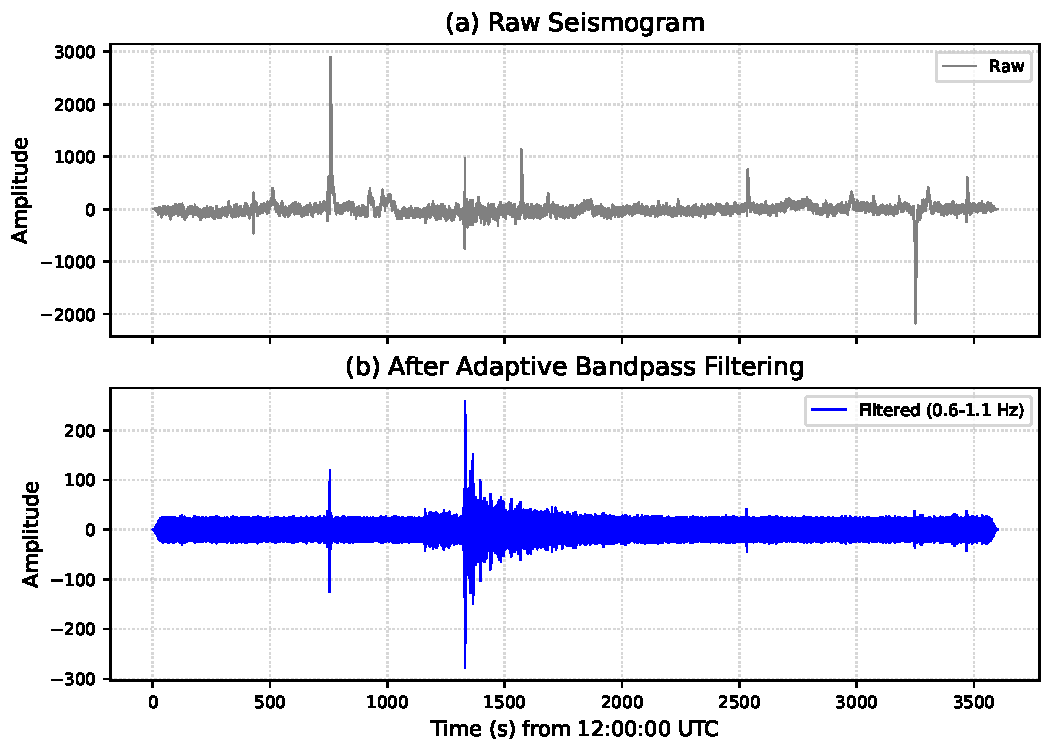
\includegraphics[width=0.9\columnwidth]{figures/fig2_adaptive_bandpass.pdf}}
                \caption{Comparison of a raw seismogram (top panel) with the same seismogram after the application 
                of the adaptively selected bandpass filter (bottom panel). The filtering aims to enhance signal 
                components within the optimal frequency range.}
                \label{fig:adaptive_filtering_comparison} 
            \end{figure}

        \subsubsection{Noise and Outlier Mitigation}
            Following the adaptive bandpass filtering, further steps are taken to mitigate noise. If resampling is
            configured , the filtered trace is resampled to a target frequency (e.g., 6.625Hz, reminiscent of Apollo-era
            sampling rates, though this is a tunable parameter). Subsequently, a threshold-based outlier removal is applied.
            Data points in the filtered trace whose absolute values exceed a multiple (e.g., 26 times) of the trace's
            standard deviation are considered outliers and are clipped to the standard deviation value. This step aims to
            reduce the impact of short, high-amplitude glitches that might otherwise distort normalization or trigger false
            STA/LTA detections.``Fig.~\ref{fig:outlier_clipping_comparison}'' illustrates the effect of this outlier clipping process.

        \begin{figure}[htbp]
            \centerline{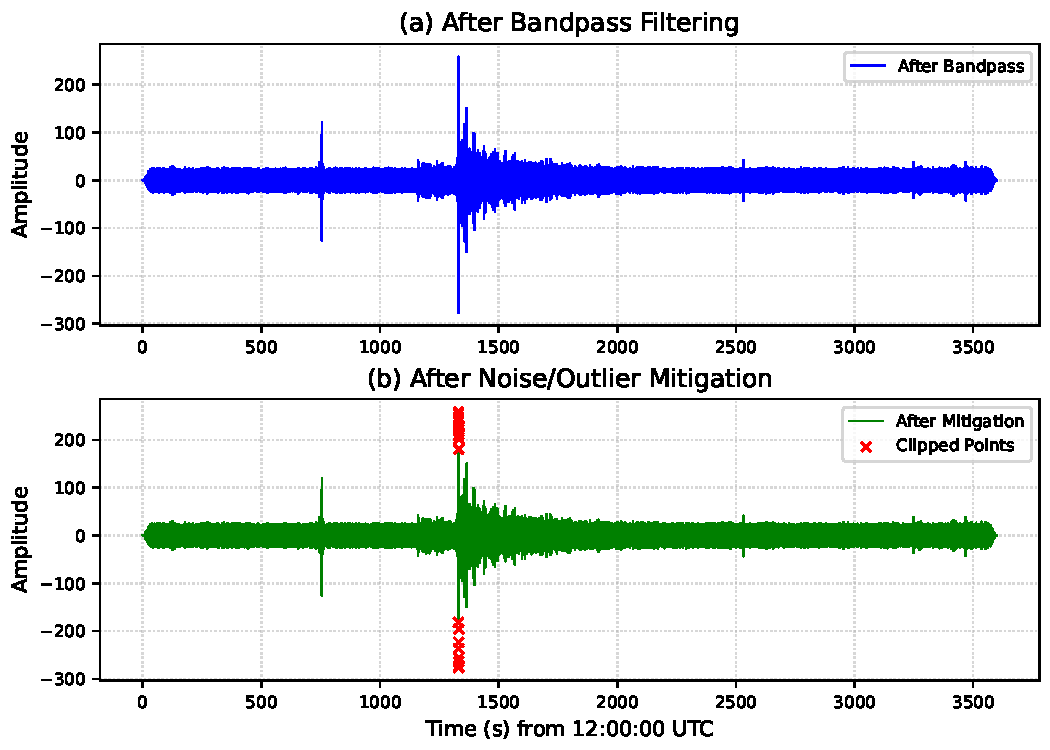
\includegraphics[width=0.9\columnwidth]{figures/fig3_mitigation.pdf}}
            \caption{Effect of outlier mitigation. The top panel shows the seismogram after bandpass filtering, 
            potentially containing high-amplitude outliers. The bottom panel displays the same seismogram after 
            the outlier clipping process, where extreme values have been attenuated.}
            \label{fig:outlier_clipping_comparison}
        \end{figure}

        \subsubsection{Data Normalization}
            After outlier removal, the filtered trace data is normalized to a consistent amplitude range,
            typically between -1 and 1. This is achieved using min-max scaling:
            
            Normalization ensures that subsequent amplitude-based detection algorithms, like STA/LTA, operate on a
            consistent scale regardless of the original signal's absolute amplitude.
                
        \subsubsection{STA\slash LTA Analysis for Initial Detection}
            Potential seismic event onsets are identified using the classic Short-Term Average to Long-Term Average
            (STA/LTA) algorithm, as implemented in Obspy \cite{Beyreuther2010}. The algorithm is applied to the absolute
            values of the normalized and filtered trace data. The lengths of the short-term window and long-term window,
            as well as the trigger-on threshold and trigger-off threshold, are configurable parameters. The trigger-off
            threshold is dynamically set based on the average of the characteristic function (CFT) generated by the
            STA/LTA algorithm. This results in a set of on-off time pairs, marking the start and end times of candidate
            detections.An example of the filtered seismogram alongside its STA/LTA characteristic function, with trigger
            points indicated, is shown in ``Fig.~\ref{fig:stalta_output}''.
            \begin{figure}[htbp]
                \centerline{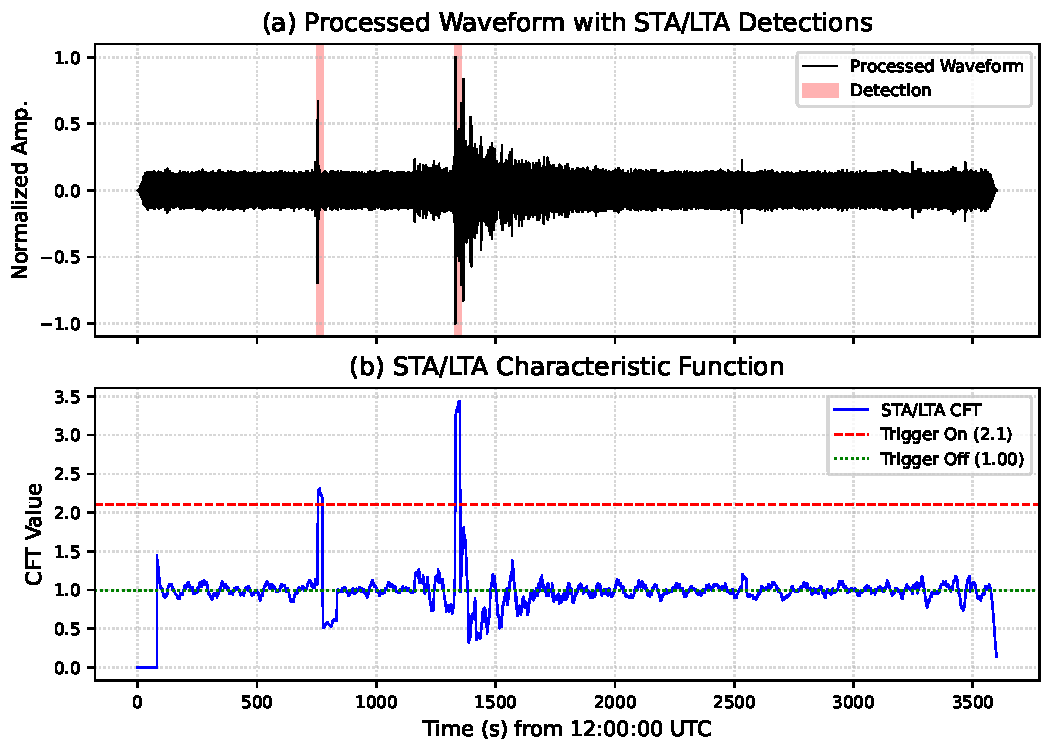
\includegraphics[width=0.9\columnwidth]{figures/fig4_stalta_detections.pdf}}
                \caption{Output of the STA/LTA analysis. The top panel shows the filtered and normalized seismogram. 
                The bottom panel displays the corresponding STA/LTA characteristic function, with red vertical 
                lines indicating trigger-on times for detected candidate events.}
                \label{fig:stalta_output}
            \end{figure}

        % \subsubsection{Candidate Pick Refinement using Characteristic Function Analysis}
        %     Not all STA/LTA triggers correspond to genuine seismic events. The Asteroseismology framework incorporates a
        %     refinement step based on the duration and number of STA/LTA triggers. Specifically, from the on-off pairs
        %     generated by STA/LTA, only those triggers where the duration (triggers[1] - triggers[0]) exceeds a certain
        %     minimum (e.g., 1200 samples, equivalent to approximately 3 minutes at 6.625 Hz if resampled) OR if the total
        %     number of triggers for the seismogram is below a certain count (e.g., less than 10) are considered for
        %     further processing. This heuristic aims to filter out very short, isolated triggers that are less likely to
        %     be significant seismic events while retaining detections from seismograms with sparse activity. Events
        %     passing this refinement are then considered qualified candidates for the subsequent machine learning stage.
        %     [Note: The provided code's characteristic function slope analysis is not explicitly implemented in the
        %     detect_events function snippet, but rather implied as a general concept in your abstract. If you have a
        %     separate code module for that, we'd need to describe it. The current code filters based on duration/count of
        %     STA/LTA triggers.]
        % \label{sec:candidate_refinement}
        %     (Detail this specific filtering mechanism based on rise/fall slopes. This is likely a novel or specifically
        %     adapted part of your conventional pipeline and should be emphasized.)
            
    \subsection{Machine Learning Stage: CNN-based Event Refinement}
        The Machine Learning-based Event Verification (MLEV) stage serves as the final arbiter in the Asteroseismology
        framework. It utilizes a Convolutional Neural Network (CNN) to classify candidate events, which have been
        pre-processed and selected by the Initial Processing and Candidate Selection (IPCS) stage (\ref{sec:ipcs}), as
        either true seismic events or noise.
    \subsubsection{Input Feature Construction for the CNN}
        For each candidate event identified by the IPCS stage, a set of specific features is prepared to serve as input
        to the CNN. This input is designed to capture both the temporal waveform characteristics and contextual
        information surrounding the potential event. The CNN takes two distinct types of inputs:

        \begin{enumerate}
            \item \textit{1D Seismogram Segments:} A fixed-length segment of the 1D seismic waveform data, centered
            around the conventionally picked arrival time, constitutes the primary input. In this study, these segments
            have a shape of (5565, 1), representing 5565 time samples for a single seismic component (e.g., vertical).
            This direct waveform input allows the CNN to learn relevant features from the time-series data itself.
            \item \textit{Auxiliary Features:} To provide additional contextual information to the network, a set of
            auxiliary features is concatenated with the processed seismogram features. These auxiliary inputs consist of
            two values: the standard deviation of the seismic signal in a window immediately preceding the picked
            arrival time, and the standard deviation in a window immediately following the picked arrival time. These
            statistical measures aim to inform the CNN about the local noise characteristics and the signal's emergence
            from the background noise. The auxiliary input thus has a shape of (2,).
        \end{enumerate}
        This dual-input approach, combining raw waveform data with engineered statistical features, distinguishes our
        method from those relying solely on time-frequency representations like spectrograms. It is intended to preserve
        fine temporal details crucial for seismic phase analysis while explicitly providing the CNN with interpretable
        contextual information.

        \subsubsection{CNN Architecture}
            The core of the MLEV stage is a CNN designed for binary classification (event vs. noise). The
            architecture, implemented using Keras \cite{Chollet2021} and visualized in ``Fig.~\ref{fig:cnn_architecture_diagram}'', is structured to process the seismogram and
            auxiliary inputs:
        
            \begin{enumerate}
                \item \textit{Seismogram Processing Branch:} The 1D seismogram input (5565, 1) is processed through a
                series of three convolutional blocks. Each block consists of a 1D Convolutional layer (Conv1D) with a
                kernel size of 3 and 'relu' activation, followed by a MaxPooling1D layer (pool size 2) for down-sampling
                and feature reduction, and a Dropout layer (rate 0.3) for regularization to prevent overfitting. The
                number of filters in the convolutional layers increases progressively: 32, 64, and 128 for the first,
                second, and third blocks, respectively. The output of the final convolutional block is flattened
                (Flatten) to produce a 1D feature vector representing the seismogram.
                
                \item \textit{Auxiliary Input Branch:} The auxiliary input (shape (2,)) is directly used without further
                convolutional processing in this branch.

                \item \textit{Combined Model:} The flattened output from the seismogram processing branch and the
                auxiliary input vector are concatenated (concatenate). This combined feature vector is then passed
                through two fully connected (Dense) layers with 'relu' activation (64 units and 32 units, respectively),
                each followed by a Dropout layer (rate 0.4) for further regularization. The final output layer is a
                single Dense unit with a 'sigmoid' activation function, producing a probability score between 0 and 1
                for binary classification.
            \end{enumerate}

            \begin{figure}[htbp]
                \centerline{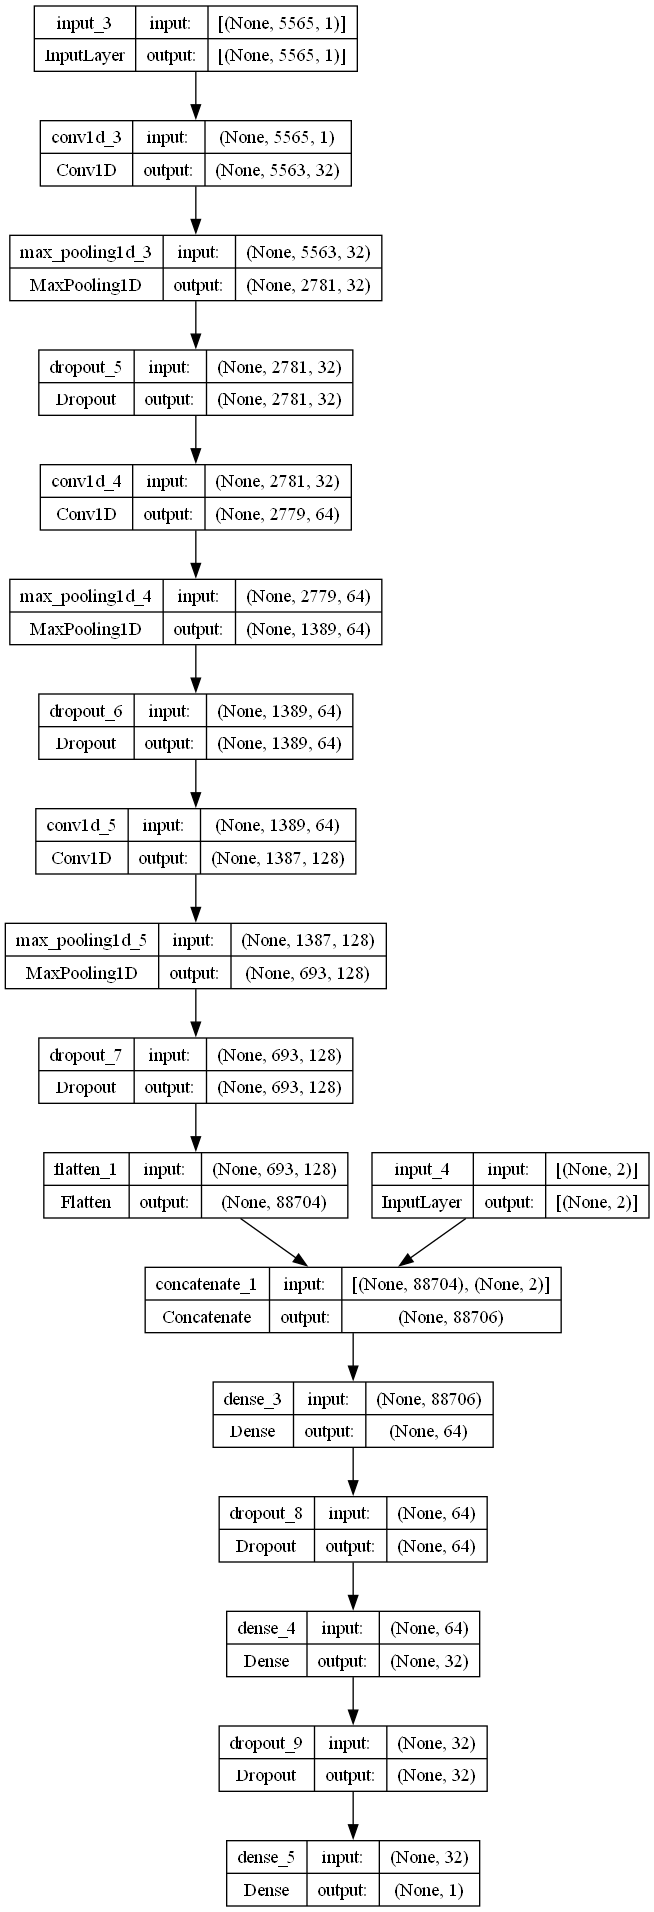
\includegraphics[width=0.7\columnwidth]{figures/CNN_Figure.png}}
                \caption{Detailed architecture of the Convolutional Neural Network (CNN) used in the MLEV stage. 
                The model takes two inputs: a 1D seismogram segment (input-3) and auxiliary features (input-4). 
                The seismogram undergoes three convolutional blocks (Conv1D, MaxPooling1D, Dropout) before being 
                flattened. The flattened seismogram features are then concatenated with the auxiliary inputs. 
                This combined representation is processed by two dense layers with dropout, leading to a final sigmoid output layer for binary classification.}
                \label{fig:cnn_architecture_diagram}
            \end{figure}
        
            The Adam optimizer \cite{Kingma2014} with a learning rate of 0.0002 is used for model compilation, and binary cross-entropy is employed as the loss function. Model performance is monitored using accuracy.
        
        \subsubsection{CNN Training and Validation}
            The CNN model is trained using curated datasets of seismic events and noise segments derived from both lunar
            (ALSEP) and Martian (InSight) missions. These datasets are prepared by concatenating multiple *.npy files
            containing the seismogram segments, corresponding auxiliary features, and binary labels (0 for noise, 1 for
            event).
        
        During training, the model is fitted for a specified number of epochs (e.g., 30) with a defined batch size
            (e.g., 32). A portion of the combined training data (e.g., 20\%) is held out for validation to monitor the
            model's generalization performance and to prevent overfitting. To address potential class imbalance in the
            training data (e.g., more noise samples than event samples), class weights (e.g., {0: 1.0, 1: 10}) are applied
            during the training process. This gives higher importance to the minority class (true events), encouraging the
            model to learn its features more effectively.
        
        \subsubsection{Event Classification and Output}
            Once the CNN model is trained and saved, it can be loaded for inference on new, unseen data. For a given
            candidate event (represented by its 1D seismogram segment and auxiliary features), the model predicts a
            single output value between 0 and 1. This value represents the probability that the input corresponds to a
            true seismic event. A predefined threshold (typically 0.5, but adjustable) is then applied to this
            probability score to make the final binary classification: if the score exceeds the threshold, the candidate
            is classified as a seismic event; otherwise, it is classified as noise.
        
        \subsection{Tunability and Adaptability of the Framework}
            The framework is designed for adaptability across diverse planetary environments and mission objectives,
            primarily through configurable parameters within its Initial Processing and Candidate Selection (IPCS)
            stage. These tunable settings allow for optimized performance whether analyzing lunar or Martian seismic
            data.
            Key tunable parameters include:
            \subsubsection{Adaptive Bandpass Filtering Controls}
                low-freq-point, high-freq-point, and frequence-window define the spectral search space and the applied
                filter width. For example, lunar data might utilize a lower frequency range (e.g., 0.2-1.0 Hz with a 0.2 Hz
                window) compared to Martian data (e.g., 0.6-4.0 Hz with a 0.5 Hz window), reflecting differing dominant
                signal frequencies and noise characteristics.
            \subsubsection{STA/LTA Detection Thresholds and Windows}
                STA and LTA length window lengths, and trigger threshold are adjusted to balance sensitivity with false
                alarm rates. Longer windows might be preferred for emergent lunar events (e.g., STA 100s, LTA 1000s), while
                shorter windows could suit sharper marsquakes (e.g., STA 20s, LTA 80s).
            \subsubsection{resampling}
                df-resample allows for a target resampling rate (e.g., 6.625 Hz) for standardization or computational efficiency.
                clipping-std-factor (e.g., 26) controls outlier removal, robustly handling transient spikes.
        
        \subsection{Datasets and Input Seismogram Preparation}
            \subsubsection{Data Sources (Lunar and Martian)}
                \begin{enumerate}[label=\alph*), leftmargin=3em]
                    \item \textit{Apollo ALSEP Data:} This dataset comprises seismic recordings from the Apollo Lunar
                    Surface Experiments Package, offering crucial insights into lunar seismicity and the Moon's internal
                    structure.
                    \item \textit{Mars InSight Mission Data:} Waveforms from NASA's Mars InSight mission, specifically from
                    the SEIS instrument, provide a wealth of information on current Martian seismic activity and atmospheric
                    phenomena.
                \end{enumerate}
                % \subsubsection{Waveform Segmentation and Initial Processing}
        \subsection{Performance Results}
        Initial evaluations of the framework demonstrate promising results. The CNN component, even with what is
        currently considered limited training data and refinement, achieved a **detection accuracy of over 80\%** on the
        test set comprising both lunar and Martian seismic signals. This indicates the model's capability to generalize
        across different planetary environments and event characteristics.
        
        Crucially, the hybrid nature of the system, particularly the pre-filtering by conventional algorithms,
        contributed to a **false positive rate of approximately 5\%**. This is a significant improvement over
        traditional methods like standalone STA/LTA, which often suffer from much higher FPRs in noisy planetary
        settings. A low FPR is vital for minimizing the transmission of non-scientific data.
        
        % Table \ref{tab:performance_summary} (placeholder) would typically summarize these key performance indicators.
        % Figure \ref{fig:roc_curve} (placeholder) would show the Receiver Operating Characteristic (ROC) curve for the
        % CNN classifier.
        
        % \begin{table}[htbp]
        %     \caption{Preliminary Performance Summary of Asteroseismology (Illustrative)}
        %     \begin{center}
        %         \begin{tabular}{|l|c|}
        %             \hline
        %             \textbf{Metric}                 & \textbf{Value} \\
        %             \hline
        %             Detection Accuracy (Events)     & $>$80\%        \\
        %             False Positive Rate (Noise)     & $\sim$5\%      \\
        %             Precision                       & [e.g., 0.85]   \\
        %             Recall                          & [e.g., 0.82]   \\
        %             F1-Score                        & [e.g., 0.83]   \\
        %             Processing Speed (1 month data) & $<$60 seconds  \\
        %             \hline
        %             \multicolumn{2}{l}{Note: Values are indicative based on abstract; actual results needed.}
        %         \end{tabular}
        %         \label{tab:performance_summary}
        %     \end{center}
        % \end{table}
        
% \section{Related Work}
% \label{sec:related_work}


% \subsection{Traditional Seismic Event Detection}
% The STA/LTA algorithm, first comprehensively described by Allen \cite{b14} and further developed by others \cite{b26},
% remains one of the most widely used methods for automatic seismic event detection due to its simplicity and
% computational efficiency. It operates by comparing the short-term average of the signal amplitude (or power) to its
% long-term average, triggering a detection when this ratio exceeds a predefined threshold. While effective for signals
% with clear onsets and high signal-to-noise ratios (SNR), STA/LTA algorithms are susceptible to false triggers from
% transient noise, instrument glitches, or complex signals with emergent onsets, particularly in the challenging noise
% environments encountered on other planetary bodies \cite{b15}.

% Template matching, or waveform cross-correlation \cite{b18}, offers higher sensitivity for detecting weak, repetitive
% seismic events, provided a known template waveform exists. This method is particularly useful for identifying families
% of similar earthquakes or moonquakes. However, its performance heavily depends on the quality and representativeness of
% the template library and can be computationally intensive for continuous scanning with a large number of templates.

% \subsection{Machine Learning in Seismology}
% The advent of machine learning has opened new frontiers in seismic data analysis. Early applications involved
% traditional ML algorithms such as Support Vector Machines (SVMs) and Random Forests for phase picking and event
% classification \cite{b19}. However, deep learning models, especially CNNs, have demonstrated superior performance in
% handling raw seismic waveforms and learning complex features directly from the data \cite{b16}.

% CNNs have been successfully applied to earthquake detection, phase picking, and magnitude estimation on Earth \cite{b17,
% b20}. Their ability to learn hierarchical features from time-series or time-frequency representations (like
% spectrograms) makes them well-suited for distinguishing subtle seismic signals from background noise.

% \subsection{Machine Learning in Planetary Seismology}
% The application of ML to planetary seismology is a more recent but rapidly growing field, driven by the unique
% challenges of these missions. The work by Civilini et al. (2021) \cite{Civilini2021} is a significant contribution in this
% area. They developed CNN models trained on spectrograms of seismic events from a single Earth station and successfully
% applied these, using transfer learning, to detect moonquakes in the Apollo Passive Seismic Experiment (PSE) and Lunar
% Seismic Profiling Experiment (LSPE) data. Their approach demonstrated the feasibility of using non-local training data
% and highlighted the potential for CNNs to catalog planetary seismicity even without prior local seismic data. They also
% introduced an "extra-arrival accuracy metric" to quantify performance on noisy lunar datasets.

Other studies have explored ML for analyzing data from the InSight mission to Mars, focusing on tasks like marsquake
detection and noise characterization \cite{b21}. The noisy operational environment of landers, combined with the diverse
and often weak seismic signals, makes robust event detection particularly challenging and an ideal candidate for
ML-driven solutions.

Our Asteroseismology framework builds upon these foundations. It acknowledges the strengths of conventional algorithms
like STA/LTA for initial, computationally cheap candidate generation, similar to some multi-stage earthquake detection
systems on Earth. However, it significantly differs from approaches like Civilini et al. \cite{favPaper} by using a
hybrid pipeline that feeds 1D waveform segments and engineered auxiliary features directly to the CNN, rather than
relying solely on spectrograms. This aims to retain fine temporal details and leverage interpretable features,
potentially enhancing both efficiency and robustness for onboard processing.



% \begin{figure}[htbp]
% \centerline{\includegraphics[width=0.8\columnwidth]{placeholder_roc.png}} % Replace with your actual figure
% \caption{Illustrative Receiver Operating Characteristic (ROC) curve for the CNN event classifier. (This is a placeholder image; please generate an ROC curve from your model's performance.)}
% \label{fig:roc_curve}
% \end{figure}

\subsection{Computational Efficiency}
The system's design prioritizes computational efficiency for potential onboard deployment. Tests conducted on a standard desktop processor (e.g., specifying CPU type and clock speed) confirmed that the Asteroseismology framework can process one month of continuous, single-component seismic data in **under 60 seconds**. This rapid processing capability is essential for near real-time analysis on resource-constrained spacecraft hardware. The efficiency stems from the fast conventional algorithms handling the bulk of the data and the lightweight CNN operating only on a filtered subset of candidate events.

% \subsection{Adaptability and Tunability}
% The six tunable parameters within the framework allow for significant adaptation to different mission requirements. For example, on a mission expecting very subtle seismic signals, the STA/LTA trigger thresholds and characteristic function parameters can be adjusted for higher sensitivity, potentially at the cost of passing more candidates to the CNN. Conversely, in a very noisy environment or when bandwidth is extremely limited, parameters can be set more conservatively to prioritize only the clearest events. This flexibility is a key advantage for diverse planetary targets and mission phases.

% \subsection{Discussion}
% The preliminary results suggest that the Asteroseismology framework offers a compelling solution for autonomous seismic
% event detection in space missions. The hybrid approach appears to strike an effective balance: the conventional
% algorithms provide a computationally cheap first pass that significantly reduces the data volume and false alarm rate
% for the CNN, while the CNN provides the sophisticated pattern recognition needed to distinguish true, often subtle,
% seismic events from complex noise.

% Compared to purely conventional methods, Asteroseismology offers substantially lower false positive rates. When compared
% to ML approaches like that of Civilini et al. \cite{favPaper}, which primarily used spectrograms as CNN input, our use
% of 1D waveforms combined with auxiliary statistical features offers a different pathway for feature extraction. While a
% direct quantitative comparison is complex without reimplementing their specific model on our exact data splits, our
% approach aims to preserve fine temporal details in the waveform and provide explicit, interpretable auxiliary features
% to the CNN, which could be advantageous for certain event types or computational constraints. The processing of data
% from both lunar (ALSEP) and Martian (InSight) missions in our training and testing pipeline also demonstrates a broader
% applicability than studies focused solely on one body.

% The current accuracy of $>$80\% with limited training is encouraging. Further expansion of the training dataset,
% including more diverse event types and noise conditions, along with more sophisticated data augmentation, is expected to
% further improve this performance. The planned integration with an AC-GAN framework (discussed in Future Work) is also
% anticipated to boost robustness.

% One limitation of the current study is the reliance on existing event catalogs for labeling, which may have their own
% biases or incompleteness. Future work could involve semi-supervised learning approaches to leverage larger amounts of
% unlabeled data.

\section{Conclusion and Future Work}
\label{sec:conclusion}
This paper has introduced Asteroseismology, an AI-driven hybrid framework for seismic event detection tailored for the
unique constraints of extra-terrestrial missions. By synergistically combining classical seismic processing algorithms
with a lightweight Convolutional Neural Network, our system demonstrates the potential for highly efficient and accurate
autonomous onboard data analysis. The framework's ability to process a month of seismic data in under a minute, coupled
with its adaptability through tunable parameters and promising initial detection accuracy of over 80\% with a low false
positive rate of approximately 5\%, underscores its suitability for optimizing data telemetry from missions to the Moon,
Mars, and beyond.

The successful application of this framework to data from both the Apollo ALSEP and Mars InSight missions indicates its
versatility in handling diverse seismic environments and instrument characteristics. This significantly reduces the
reliance on manual or semi-automatic ground-based processing, enabling faster scientific turnaround and more efficient
use of limited deep-space communication resources.

Future work can focus on several key areas to further enhance the framework:
\begin{enumerate}
    \item \textbf{CNN Architecture and Training Refinement:} Exploring more advanced CNN architectures and expand
    the training dataset significantly. This will include incorporating a wider variety of seismic event types, noise
    profiles, and employing sophisticated data augmentation techniques to improve generalization and robustness.
    \item \textbf{Integration with Auxiliary Classifier Conditional GAN (AC-GAN):} A primary future development is the
    refinement of the CNN within an AC-GAN framework \cite{b22}. AC-GANs can be used to generate more realistic
    synthetic seismic data for training, particularly for rare event types, and can also improve the classifier's
    ability to distinguish subtle differences between event classes and noise by simultaneously learning to classify and
    generate data. This is expected to further improve detection reliability and reduce false positives.
    \item \textbf{Enhanced Auxiliary Features:} We will investigate the inclusion of a richer set of physics-informed
    auxiliary features for the CNN, derived from more detailed analysis of the candidate event waveforms by the
    conventional algorithms.
    \item \textbf{Onboard Implementation Prototyping:} Efforts will be made to prototype the system on hardware
    representative of spacecraft processors (e.g., FPGAs or radiation-hardened CPUs) to rigorously evaluate its
    performance under realistic resource constraints.
    \item \textbf{Expansion to Other Planetary Bodies:} While currently focused on lunar and Martian data, the
    framework's adaptable design makes it a candidate for future missions to other seismically active bodies like Europa
    or Titan, with appropriate tuning and training data.
\end{enumerate}

In conclusion, the framework represents a significant step towards enabling more autonomous and scientifically
productive planetary seismology missions. By intelligently managing data at the source, it helps to overcome critical
mission constraints, paving the way for deeper and more comprehensive exploration of the internal structures of
celestial bodies in our solar system.

\section*{Acknowledgment}
The authors would like to thank the NASA Planetary Data System (PDS) for providing access to the Apollo ALSEP and Mars InSight mission data. We also acknowledge the developers of open-source software packages used in this research, including [mention specific libraries like Obspy, TensorFlow/Keras, Scikit-learn if used].

\begin{thebibliography}{00}
    \bibitem{Civilini2021} F. Civilini, R.C. Weber, Z. Jiang, D. Phillips, and W. David Pan, ``Detecting moonquakes using convolutional neural networks, a non-local training set, and transfer learning,'' \emph{Geophys. J. Int.}, vol. 225, no. 3, pp. 2120--2134, Mar. 2021.
    \bibitem{Lognonne2005}  P. Lognonné, ``Planetary seismology,'' \emph{Annu. Rev. Earth Planet. Sci.}, vol. 33, pp. 571--604, May 2005.
    \bibitem{Lognonne2019} P. Lognonné, W. B. Banerdt, V. Dehant, et al., ``SEIS: The seismic experiment for internal structure of InSight,'' \emph{Space Sci. Rev.}, vol. 215, Art. no. 12, Feb. 2019, doi: 10.1007/s11214-018-0574-6.
    \bibitem{Nakamura1982} Y. Nakamura, G. V. Latham, and H. J. Dorman, ``Apollo lunar seismic experiment – Final summary,'' \emph{J. Geophys. Res.}, vol. 87, no. S01, p. A117, 1982.
    \bibitem{Nakamura1981} Y. Nakamura, ``Lunar seismicity and the internal structure of the Moon,'' \emph{J. Geophys. Res.}, vol. 86, no. B10, pp. 9413--9424, Oct. 1981.
    \bibitem{Lorenz2015} R. D. Lorenz, ``Energy cost of acquiring and transmitting science data on deep-space missions,'' \emph{J. Spacecr. Rockets}, vol. 52, no. 6, pp. 1693--1697, Nov. 2015.
    \bibitem{Nunn2020} C. Nunn, R. F. Garcia, Y. Nakamura, et al., ``Lunar seismology: A data and instrumentation review,'' \emph{Space Sci. Rev.}, vol. 216, no. 89, pp. 1--37, 2020.
    \bibitem{Dainty1981} A. Dainty and M. Toksöz, ``Seismic codas on the Earth and the Moon: A comparison,'' \emph{Phys. Earth Planet. Inter.}, vol. 26, no. 4, pp. 250--260, 1981.
    \bibitem{Garcia2019} R. F. Garcia, A. Khan, M. Drilleau, et al., ``Lunar seismology: An update on interior structure models,'' \emph{Space Sci. Rev.}, vol. 215, no. 50, pp. 1--50, 2019.
    \bibitem{Weber2011} R. C. Weber, P. Y. Lin, E. J. Garnero, Q. Williams, and P. Lognonné, ``Seismic detection of the lunar core,'' \emph{Science}, vol. 331, no. 6015, pp. 309--312, Jan. 2011.
    \bibitem{Anderson1977} D. L. Anderson, W. F. Miller, G. V. Latham, Y. Nakamura, M. N. Toksöz, A. M. Dainty, F. K. Duennebier, A. R. Lazarewicz, R. L. Kovach, and T. C. D. Knight, ``Seismology on Mars,'' \emph{J. Geophys. Res.}, vol. 82, no. 28, pp. 4524--4546, 1977.
    \bibitem{Banerdt2020} W. B. Banerdt et al., ``Initial results from the InSight mission on Mars,'' \emph{Nature Geoscience}, vol. 13, pp. 183--189, Mar. 2020.
    \bibitem{Giardini2020} D. Giardini et al., ``The seismicity of Mars,'' \emph{Nature Geoscience}, vol. 13, pp. 205--212, 2020.
    \bibitem{Clinton2021} J. F. Clinton et al., ``The Marsquake catalogue from InSight, sols 0--478,'' \emph{Phys. Earth Planet. Inter.}, vol. 310, Art. no. 106595, 2021
    \bibitem{MousaviBeroza2022} S. M. Mousavi and G. C. Beroza, ``Deep-learning seismology,'' \emph{Science}, vol. 377, no. 6606, p. eabm4470, Aug. 2022, doi: 10.1126/science.abm4470.   
    \bibitem{Beyreuther2010} M. Beyreuther, R. Barsch, L. Krischer, T. Megies, Y. Behr, and J. Wassermann, "ObsPy: A Python toolbox for seismology," Seismological Research Letters, vol. 81, no. 3, pp. 530-533, 2010.
    \bibitem{Chollet2021} F. Chollet, "Deep Learning with Python," Simon and Schuster, 2021.
    \bibitem{Kingma2014} D. P. Kingma and J. Ba, "Adam: A method for stochastic optimization," arXiv preprint arXiv:1412.6980, 2014.
    % \bibitem{b3} I. S. Jacobs and C. P. Bean, ``Fine particles, thin films and exchange anisotropy,'' in Magnetism, vol. III, G. T. Rado and H. Suhl, Eds. New York: Academic, 1963, pp. 271--350. 
    % \bibitem{b4} K. Elissa, ``Title of paper if known,'' unpublished. 
    % \bibitem{b5} R. Nicole, ``Title of paper with only first word capitalized,'' J. Name Stand. Abbrev., in press. 
    % \bibitem{b6} Y. Yorozu, M. Hirano, K. Oka, and Y. Tagawa, ``Electron spectroscopy studies on magneto-optical media and plastic substrate interface,'' IEEE Transl. J. Magn. Japan, vol. 2, pp. 740--741, August 1987 [Digests 9th Annual Conf. Magnetics Japan, p. 301, 1982]. 
    % \bibitem{b7} M. Young, The Technical Writer's Handbook. Mill Valley, CA: University Science, 1989.
    % \bibitem{b8} S. C. Solomon et al., ``New perspectives on ancient Mars,'' \emph{Science}, vol. 307, no. 5713, pp. 1214--1220, Feb. 2005.
    % \bibitem{b9} P. Lognonné, ``Planetary seismology,'' \emph{Annu. Rev. Earth Planet. Sci.}, vol. 33, pp. 571--604, May 2005.
    % \bibitem{b12} P. Lognonné et al., ``SEIS: Insight’s seismic experiment for internal structure of Mars,'' \emph{Space Sci. Rev.}, vol. 215, no. 12, Feb. 2019.
    % \bibitem{b13} R. D. Lorenz, ``Energy cost of acquiring and transmitting science data on deep-space missions,'' \emph{J. Spacecr. Rockets}, vol. 52, no. 6, pp. 1693--1697, Nov. 2015.
    % \bibitem{b14} R. Allen, ``Automatic earthquake recognition and timing from single traces,'' \emph{Bull. Seismol. Soc. Am.}, vol. 68, no. 5, pp. 1521--1532, Oct. 1978.
    % \bibitem{b15} M. P. Panning et al., ``Expected seismicity and the seismic noise environment of Europa,'' \emph{J. Geophys. Res. Planets}, vol. 123, no. 1, pp. 163--179, Jan. 2018.
    % \bibitem{b16} T. Perol, M. Gharbi, and M. Denolle, ``Convolutional neural network for earthquake detection and location,'' \emph{Sci. Adv.}, vol. 4, no. 2, p. e1700578, Feb. 2018.
    % \bibitem{b17} Z. E. Ross, M. J. Meier, and E. Hauksson, ``Generalized seismic phase detection with deep learning,'' \emph{Bull. Seismol. Soc. Am.}, vol. 108, no. 5A, pp. 2894--2901, Oct. 2018.
    % \bibitem{b18} G. C. Beroza and S. G. Shelly, ``Detecting and characterizing earthquake swarms,'' \emph{Science}, vol. 319, no. 5865, pp. 906--909, Feb. 2008. (Note: this is a review mentioning template matching, original template matching papers are older, e.g., Gibbons \& Ringdal 2006)
    % \bibitem{b19} S. Mostafa, M. R. Zare, and S. M. J. Aleali, ``Seismic signal classification using support vector machine and particle swarm optimization,'' \emph{J. Seismol.}, vol. 19, pp. 619--630, 2015.
    % \bibitem{b20} W. J. N. R. Mousavi, S. M., Horton, S. P., et al., ``CRED: A deep residual network of convolutional and recurrent units for earthquake signal detection,'' \emph{Sci. Rep.}, vol. 9, no. 1, p. 10267, Jul. 2019.
    % \bibitem{b21} C. Clinton et al., ``The Marsquake catalogue from InSight, S01 to S08,'' \emph{Phys. Earth Planet. Inter.}, vol. 310, p. 106595, Jan. 2021.
    % \bibitem{b22} A. Odena, C. Olah, and J. Shlens, ``Conditional image synthesis with auxiliary classifier GANs,'' in \emph{Proc. Int. Conf. Mach. Learn. (ICML)}, 2017, pp. 2642--2651.
    % \bibitem{b26} F. Baer, M., \& Kradolfer, U. (1987). An automatic phase picker for local and teleseismic events. \emph{Bulletin of the Seismological Society of America}, 77(4), 1437-1445.


\end{thebibliography}

\end{document}